
\section{Bivektoren
\label{geoalgebra:section:bivektoren}}
\kopfrechts{Bivektoren}
\subsection{Idee}
\label{geoalgebra:section:bivektoren:idee}
\newcommand{\vone}{\color{red}\mathbf{v}_1\color{black}}
\newcommand{\vtwo}{\color{blue}\mathbf{v}_2\color{black}}
Durch das Wedgeprodukt zwischen $\vone$ und $\vtwo$ erhalten wir
den
Bivektor $\vone \wedge \vtwo$. Einen Bivektor können wir uns als \emph{orientierte Fläche}, die zwischen den beiden Vektoren aufgespannt
wird, vorstellen (siehe \autoref{geoalgebra:fig:bivektor-als-flaeche}).
\begin{figure}
  \begin{center}
\begin{tikzpicture}[>=latex, thick]
  \draw[step=.5cm,gray,very thin] (-0.25,-0.25) grid (5.25,4.25);
  \coordinate (O) at (0,0);
  \coordinate (A) at (3,1);
  \coordinate (B) at (2,3);
  \coordinate (C) at ($(A)+(B)$);

  \fill[blue!30,opacity=0.7] (O) -- (A) -- (C) -- (B) -- cycle;

  \draw[thick,->,darkred] (O) -- (A) node[midway,below] {$\acolored$};
  \draw[thick,->,blue] (O) -- (B) node[midway,left] {$\bcolored$};
  \draw[dashed] (A) -- (C);
  \draw[dashed] (B) -- (C);

  \node (K) at ($0.25*(O)+0.25*(A)+0.25*(B)+0.25*(C)$)
    {$\color{darkred}\acolored \wedge \bcolored$};
  \draw[thick,->] (K) ++(0.6,0) arc (0:270:0.6);
\end{tikzpicture}

  \end{center}
  \caption{Bivektor als orientierte Fläche}\label{geoalgebra:fig:bivektor-als-flaeche}
\end{figure}

\subsection{Bivektoren als orientierte Fläche}
Es ist wichtig, dass wir uns die Idee einer orientierten Fläche
verinnerlichen. Wie wir bereits in \autoref{geoalgebra:section:bivektoren:idee} gesehen haben,
gibt das Wedgeprodukt $\vone \wedge \vtwo$
einen Bivektor, der die Fläche zwischen den beiden Vektoren als
eine \emph{im Gegenuhrzeigersinn orientierte Fläche} repräsentiert.
Wir können uns vorstellen, als ob wir den Vektor $\vone$
am Vektor $\vtwo$ ``aufspannen'' (siehe \autoref{geoalgebra:fig:aufspannende-flaeche-v1-v2})

\begin{figure}
\begin{center}
\begin{tikzpicture}[>=latex, thick]
  \draw[step=.5cm,gray,very thin] (-0.25,-0.25) grid (5.25,4.25);
  \coordinate (O) at (0,0);
  \coordinate (A) at (3,1);
  \coordinate (B) at (2,3);
  \coordinate (C) at ($(A)+(B)$);
  \coordinate (M_AC) at ($0.5*(A)+0.5*(C)$);
  \coordinate (M_OB) at ($0.5*(O)+0.5*(B)$);

  \fill[blue!30,opacity=0.7] (O) -- (A) -- (M_AC) -- (M_OB) -- cycle;

  \draw[thick,->,darkred] (O) -- (A) node[midway,below] {$\acolored$};
  \draw[thick,->,blue] (O) -- (B) node[midway,left] {$\bcolored$};
  \draw[dashed] (A) -- (C);
  \draw[dashed] (B) -- (C);
  \draw[thick,->,blue] (3.7, 1.9) -- (4.3, 2.8);


  \node (K) at ($0.25*(O)+0.25*(A)+0.25*(B)+0.25*(C)$)
    {$\acolored \wedge \bcolored$};
  \draw[thick,->] (K) ++(0.6,0) arc (0:270:0.6);
\end{tikzpicture}

\begin{tikzpicture}[>=latex]
  \draw[step=.5cm,gray,very thin] (-0.25,-0.25) grid (5.25,4.25);
  \coordinate (0) at (0, 0);
  \coordinate (A) at (3, 1);
  \coordinate (B) at (2, 3);
  \coordinate (C) at ($(A) + (B)$);
  \fill[blue!30, opacity=0.7] (0) -- (A) -- (C) -- (B) -- cycle;

  \draw[thick, ->, darkred] (0) -- (A) node[midway,below] {$\acolored$};
  \draw[thick, ->, blue] (0) -- (B) node[midway,left] {$\bcolored$};
  \draw[dashed] (A) -- (C);
  \draw[dashed] (B) -- (C);
  \node (K) at ($0.25*(0)+0.25*(A)+0.25*(B)+0.25*($(C)$)$)
  {$\acolored \wedge \bcolored$};
\draw[thick,->] (K) ++(0.6,0) arc (0:270:0.6);
\end{tikzpicture}

\end{center}
  \caption{Vektor $\vone$ wird an $\vtwo$ aufgespannt}\label{geoalgebra:fig:aufspannende-flaeche-v1-v2}
\end{figure}


Analog dazu stellen wir uns vor, dass wir beim Bivektor $\vtwo \wedge \vone$ den Vektor
$\vtwo$ am Vektor $\vone$ aufspannen (siehe \autoref{geoalgebra:fig:aufspannende-flaeche-v2-v1}).
In diesem Fall entsteht eine im Uhrzeigersinn orientierte Fläche mit demselben
Flächeninhalt. Laut Axiom \eqref{geoalgebra:eq:antikommutativ} ist das Wedgeprodukt
\emph{antikommutativ}, d.h. $\vone \wedge \vtwo = -\vtwo \wedge \vone$. Das Vorzeichen bestimmt also,
wie die Fläche orientiert ist.

\begin{figure}
\begin{center}
\begin{tikzpicture}[>=latex]
\draw[step=.5cm,gray,very thin] (-0.25,-0.25) grid (5.25,4.25);
\coordinate (O) at (0,0);
\coordinate (A) at (3,1);
\coordinate (B) at (2,3);
\coordinate (C) at ($(A)+(B)$);
\coordinate (M_BC) at ($0.5*(B)+0.5*(C)$);
\coordinate (M_OA) at ($0.5*(O)+0.5*(A)$);

\fill[red!30,opacity=0.7] (O) -- (A) -- (M_OA) -- (M_BC) -- (B) -- cycle;

\draw[thick,->,red] (O) -- (A) node[midway,below] {$\vone$};
\draw[thick,->,blue] (O) -- (B) node[midway,left] {$\vtwo$};
\draw[dashed] (A) -- (C);
\draw[dashed] (B) -- (C);
\draw[thick,->,red] (2.85,3.44) -- (3.75,3.74);

\node (K) at ($0.25*(O)+0.25*(A)+0.25*(B)+0.25*(C)$)
  {$\vtwo \wedge \vone$};
\draw[thick,->] (K) ++(0.6,0) arc (0:-270:0.6);
\end{tikzpicture}

\begin{tikzpicture}[>=latex]
  \draw[step=.5cm,gray,very thin] (-0.25,-0.25) grid (5.25,4.25);
  \coordinate (0) at (0, 0);
  \coordinate (A) at (3, 1);
  \coordinate (B) at (2, 3);
  \coordinate (C) at ($(A) + (B)$);
  \fill[red!30, opacity=0.7] (0) -- (A) -- (C) -- (B) -- cycle;

  \draw[thick, ->, red] (0) -- (A) node[midway,below] {$\acolored$};
  \draw[thick, ->, blue] (0) -- (B) node[midway,left] {$\bcolored$};
  \draw[dashed] (A) -- (C);
  \draw[dashed] (B) -- (C);
  \node (K) at ($0.25*(O)+0.25*(A)+0.25*(B)+0.25*(C)$)
    {$\bcolored \wedge \acolored$};
  \draw[thick,->] (K) ++(0.6,0) arc (0:-270:0.6);
\end{tikzpicture}

\end{center}
  \caption{$\vtwo$ wird an $\vone$ aufgespannt}\label{geoalgebra:fig:aufspannende-flaeche-v2-v1}
\end{figure}

Eine positive, orientierte Fläche ist generell einem Umlaufsinn \emph{im Uhrzeigersinn}
zuzuordnen, eine negative, orientierte Fläche bedeutet ein Umlaufsinn \emph{im Gegenuhrzeigersinn}.


\subsection{Rechenbeispiel mit Zahlen}
\label{geoalgebra:section:example}

Wir nehmen an, dass 
\begin{equation}
  \begin{aligned}
    &\mathbf{a} &= \begin{pmatrix} 3 \\ 1 \end{pmatrix} = 3 \eone + \etwo \\
    \text{und}\quad
    &\mathbf{b} &= \begin{pmatrix} 1 \\ 2 \end{pmatrix} = \eone + 2 \etwo.
  \end{aligned}
\end{equation}
Das Wedgeprodukt zwischen den beiden Vektoren ergibt
\begin{equation}
  \begin{aligned}
    \mathbf{a} \wedge \mathbf{b} &= (3 \eone + \etwo) \wedge (\eone + 2 \etwo) \\
    &= 5 \eone \wedge \etwo.
  \end{aligned}
\end{equation}
Die Fläche im aufgespannten Parallelogramm ist $5$ und im Gegenuhrzeigersinn orientiert.

\subsection{Äquivalente Bivektoren}
Da Bivektoren orientierte Flächen sind, sind sie nicht eindeutig. Es gibt unendlich viele mögliche Kombinationen von Vektoren,
die denselben Bivektor erzeugen.

Ein ganz einfaches Beispiel von einem äquivalenten Bivektor erhalten wir, wenn wir in einem Wedgeprodukt zweier Vektoren einen strecken
und den anderen stauchen. Dies lässt sich bereits aus unseren Axiomen herleiten.

{
\renewcommand{\a}{\mathbf{a}}
\renewcommand{\b}{\mathbf{b}}
\begin{beispiel}
Sei
  \begin{align*}
    \a &= \begin{pmatrix} 3 \\ 1 \end{pmatrix} \\
    \b &= \begin{pmatrix} 1 \\ 2 \end{pmatrix}
  \end{align*}
Das Wedgeprodukt zwischen $\a$ und $\b$ ergibt
  \begin{equation}
    \a \wedge \b = 5 \eone \wedge \etwo.
  \end{equation}

  Wir strecken $\a$ und stauchen $\b$ um denselben Faktor $2$. Durch die Bilinearität (\eqref{geoalgebra:eq:bilinear}) ergibt
  \begin{equation}
    2 \a \wedge \frac{1}{2} \b = 2 \frac{1}{2} \a \wedge \b = \a \wedge \b.
  \end{equation}



\begin{figure}
  \begin{center}
\begin{tikzpicture}[>=latex]
  \draw[step=.5cm,gray,very thin] (-0.25,-0.25) grid (4.25,4.25);
  \coordinate (O) at (0,0);
  \coordinate (A) at (3,1);
  \coordinate (B) at (1,2);
  \coordinate (C) at ($(A)+(B)$);

  \fill[blue!30,opacity=0.7] (O) -- (A) -- (C) -- (B) -- cycle;

  \draw[thick,->,red] (O) -- (A) node[midway,below] {$\a$};
  \draw[thick,->,blue] (O) -- (B) node[midway,left] {$\b$};
  \draw[dashed] (A) -- (C);
  \draw[dashed] (B) -- (C);

  \node (K) at ($0.25*(O)+0.25*(A)+0.25*(B)+0.25*(C)$)
    {$\a \wedge \b$};
  \draw[thick,->] (K) ++(0.5,0) arc (0:270:0.5);
\end{tikzpicture}

\begin{tikzpicture}[>=latex, thick]
  \draw[step=.5cm,gray,very thin] (-0.25,-0.25) grid (2.25,3.25);
  \coordinate (O) at (0,0);
  \coordinate (A) at (2,0);
  \coordinate (B) at (0,5/2);
  \coordinate (C) at ($(A)+(B)$);

  \fill[blue!30,opacity=0.7] (O) -- (A) -- (C) -- (B) -- cycle;

  \draw[thick,->,darkred] (O) -- (A) node[midway,below] {$2 \eone$};
  \draw[thick,->,blue] (O) -- (B) node[midway,left] {$\frac{5}{2} \etwo$};
  \draw[dashed] (A) -- (C);
  \draw[dashed] (B) -- (C);

\end{tikzpicture}

  \end{center}
  \caption{Beide Bivektoren sind äquivalent mit Fläche $5$}\label{geoalgebra:fig:bivektor-als-flaeche}.
\end{figure}
\end{beispiel}

Derselbe Bivektor kann aber auch über Vektoren in andere Richtungen erreicht werden, z.B. über die Standardbasisvektoren $\eone$ und $\etwo$ (siehe \autoref{geoalgebra:fig:equivalent-bivectors-unit-vectors}).

\begin{figure}
\begin{center}
\begin{tikzpicture}[>=latex]
  \draw[step=.5cm,gray,very thin] (-0.25,-0.25) grid (4.25,4.25);
  \coordinate (O) at (0,0);
  \coordinate (A) at (3,1);
  \coordinate (B) at (1,2);
  \coordinate (C) at ($(A)+(B)$);

  \fill[blue!30,opacity=0.7] (O) -- (A) -- (C) -- (B) -- cycle;

  \draw[thick,->,red] (O) -- (A) node[midway,below] {$\a$};
  \draw[thick,->,blue] (O) -- (B) node[midway,left] {$\b$};
  \draw[dashed] (A) -- (C);
  \draw[dashed] (B) -- (C);

  \node (K) at ($0.25*(O)+0.25*(A)+0.25*(B)+0.25*(C)$)
    {$\a \wedge \b$};
  \draw[thick,->] (K) ++(0.5,0) arc (0:270:0.5);
\end{tikzpicture}

\begin{tikzpicture}[>=latex, thick]
  \draw[step=.5cm,gray,very thin] (-0.25,-0.25) grid (2.25,3.25);
  \coordinate (O) at (0,0);
  \coordinate (A) at (2,0);
  \coordinate (B) at (0,5/2);
  \coordinate (C) at ($(A)+(B)$);

  \fill[blue!30,opacity=0.7] (O) -- (A) -- (C) -- (B) -- cycle;

  \draw[thick,->,darkred] (O) -- (A) node[midway,below] {$2 \eone$};
  \draw[thick,->,blue] (O) -- (B) node[midway,left] {$\frac{5}{2} \etwo$};
  \draw[dashed] (A) -- (C);
  \draw[dashed] (B) -- (C);

\end{tikzpicture}

  \caption{Bivektoren der Fläche $5$ gebildet durch die Standardbasisvektoren}
  \label{geoalgebra:fig:equivalent-bivectors-unit-vectors}
\end{center}
\end{figure}

}


\subsection{Bivektoren im dreidimensionalen Raum}
Bivektoren sind in allen Dimensionen genauso orientierte Flächen wie in zwei Dimensionen.
Statt, dass wir jedoch das Resultat einfach so erhalten, erhalten wir \emph{Projektionen}
auf alle von den Standardbasisvektoren aufgespannten Ebenen.

In \eqref{geoalgebra:eq:wedgeprodukt-dreidimensional} haben wir das Wedgeprodukt zwischen zwei Vektoren
in drei Dimensionen bereits hergeleitet. Wir erhielten drei Summanden aus Wedgeprodukten mit skalaren Faktoren
\begin{align*}
&(a_1 b_2 - a_2 b_1) \eone \wedge \etwo \\
  &+(a_2 b_3 - a_3 b_2) \etwo \wedge \ethree \\
  &+(a_3 b_1 - a_1 b_3) \ethree \wedge \eone.
\end{align*}
Der Term $a_1 b_2 - a_2 b_1$ ist der Flächeninhalt der \emph{Projektion} (oder des ``Schattens'') des aufgespannten Parallelogramms auf die $\eone$-$\etwo$-Ebene.
Analog dazu ist $a_2 b_3 - a_3 b_2$ der Flächeninhalt der Projektion auf die $\etwo$-$\ethree$-Ebene und $a_3 b_1 - a_1 b_3$ der Flächeninhalt
der Projektion auf die $\ethree$-$\eone$-Ebene (siehe \autoref{geoalgebra:fig:bivectors-3d}).

\begin{figure}[h]
  \centering
  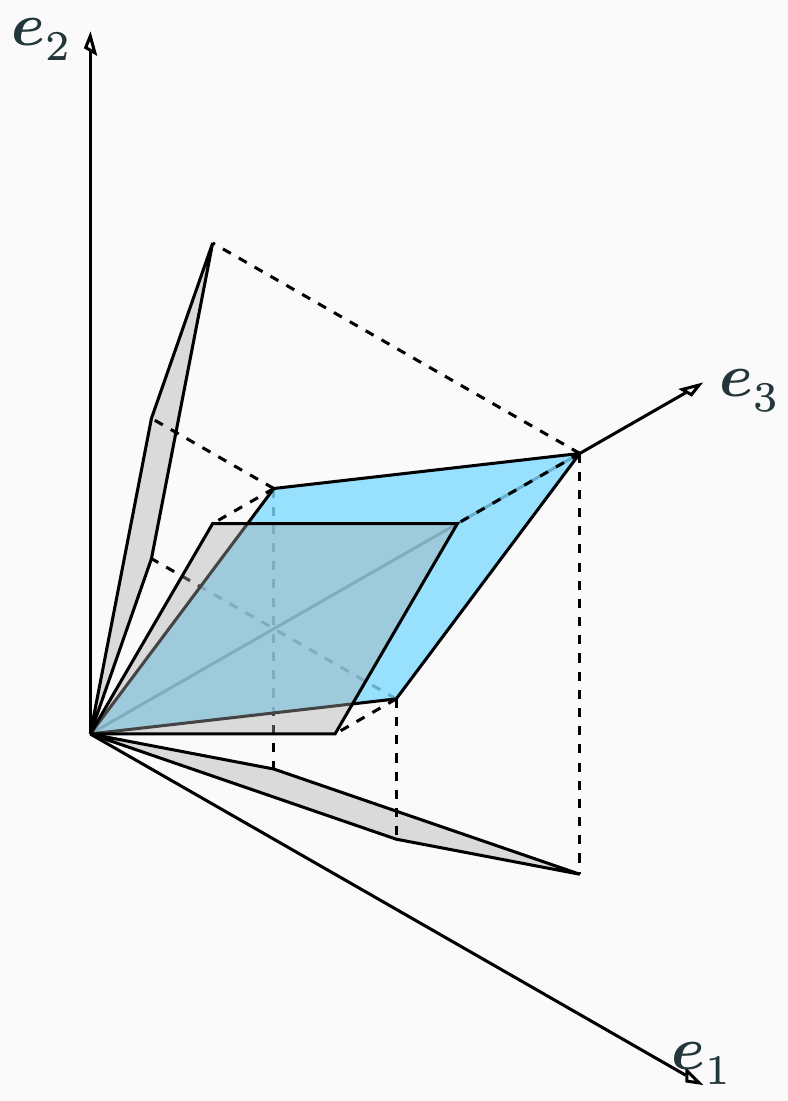
\includegraphics[width=0.4\textwidth]{papers/geoalgebra/assets/bivectors-3d.png}
  \caption{Bivektoren im dreidimensionalen Raum}
  \label{geoalgebra:fig:bivectors-3d}
\end{figure}

\subsection{Bivektoren als algebraische Struktur}
Bisher wurde besonders auf geometrische Vorstellungen eines Bivektors eingegangen. Vor dem nächsten Thema sollte hier noch kurz
auf die algebraische Struktur eines Bivektors eingegangen werden. Das Wedgeprodukt zweier zweidimensionalen Vektoren ergibt
einen Bivektor mit genau einer Komponente. Das Wedgeprodukt zwischen zwei dreidimensionalen Vektoren ergibt einen Bivektor mit drei Komponenten
und das Wedgeprodukt zwischen
zwei vierdimensionalen Vektoren ergibt sechs.

Die Anzahl Komponenten, die aus einem Bivektor resultieren, hängt also von der Dimension des Vektorraums ab, den wir betrachten.
Wie in \eqref{geoalgebra:eq:2d-wedgeproduct} bereits erkannt, fallen die Terme, welche Wedgeprodukte von gleichen Vektoren $\mathbf{v}_i \wedge \mathbf{v}_i$ beinhalten,
immer weg, da diese Produkte $0$ ergeben. Ausserdem werden vertauschte Reihenfolgen einfach negiert und zusammengefasst: 
\begin{equation}
  \lambda \mathbf{v}_i \wedge \mathbf{v}_j + \mu \mathbf{v}_j \wedge \mathbf{v_i} = \lambda \mathbf{v}_i \wedge \mathbf{v}_j - \mu \mathbf{v}_i \wedge \mathbf{v}_j = (\mu - \lambda) \mathbf{v}_i \wedge \mathbf{v}_j
\end{equation}
Wir erhalten also für jede Kombination von verschiedenen Basisvektoren eines Vektorraums eine Komponente.
\begin{satz}
Sei $N$ die Dimension des Vektorraumes. Die Dimension $K$ des Raums der Bivektoren berechnet sich als
  \begin{equation}
    \label{geoalgebra:eq:components-bivectors}
    K = \binom{N}{2}.
  \end{equation}
\end{satz}


